\documentclass{article}

%%%%%%%%%%%%%%%%%%%%%%%%%%%%%%%%%%
% the following makes the preamble
%%%%%%%%%%%%%%%%%%%%%%%%%%%%%%%%%%

% package for equaiton*, which to remove
% automatic numbering in math equations
\usepackage{amsmath}

% package for \includegraphics[]{}
\usepackage{graphicx}

% package for subfigures
\usepackage{subcaption}

% package for change spacing
% eg.
% \doublespacing
% \singlespacing
\usepackage{setspace}


% example for footnote citation
% package for citing literature in footnotes
% \usepackage[backend=bibtex,style=verbose-trad2]{biblatex}
% \bibliography{reference} 

% package to tell how many digital places it should display
% used in table example by changing column alignment from c to S
\usepackage{siunitx}
\sisetup{
    round-mode = places, % rounds numbers
    round-precision = 2,  % up to 2 places
}

% multirow in table example
\usepackage{multirow}

% table beauty package for \hline replacement
\usepackage{booktabs}

% To display tables on several pages
\usepackage{longtable}

% pgf/tikz for beautiful graphics especially diagram
\usepackage{tikz}


% adding cliable links
\usepackage{hyperref}

\title{Latex Tutorial}
\date{2021-01-10}
\author{Bear5}

%%%%%%%% end of preamble %%%%%%%%%
%%%%%%%%%%%%%%%%%%%%%%%%%%%%%%%%%%


\begin{document}
% turn off the page number
\pagenumbering{gobble}

% page for title
\maketitle
\newpage

% page for table of content
\tableofcontents
\newpage

\doublespacing
% page for list of figures
\listoffigures
\singlespacing
\newpage

\listoftables
\newpage

% turn on page numbering
% gobble, arabic, roman
\pagenumbering{arabic}



\section{Structure}
Hello World!

\subsection{Subsection}
This is a subsection

\subsubsection{Subsubsection}
this is a subsubsection


\paragraph{Paragraph}
Some paragraph text

\subparagraph{Subparagraph}
More subparagraph text .

\newpage
\section{Section 2}


\subsection{Math}
\begin{equation}
    f(x) = x^2
\end{equation}

\begin{equation*}
    \dot{x}= -x + 2x
\end{equation*}

\begin{align*}
    f(x) &= x^2 \\
    \dot{x} &= -x + 2x
\end{align*}

\begin{align*}
    f(x) &= x^2 \\
    g(x) &= \frac{1}{\sqrt{x}} \\
    h(x) &= \int^a_b \frac{1}{3}x^3dx \\
    \left[\begin{matrix}
        1 & 0 \\
        0 & 1
    \end{matrix}\right]^T & =
    \left[\begin{matrix}
            1 & 0 \\
            0 & 1
          \end{matrix}\right]
\end{align*}

This formula $f(x) = x^2$ is an example of inline math


\subsection{Figure}
\begin{figure}
   \includegraphics[width=\linewidth]{porcupine.JPG} 
   \caption{Porcupine.}
   \label{fig:porcupine}
\end{figure}
Figure \ref{fig:porcupine} shows the beauty of Porcupine mountain


\begin{figure}
    \centering
    \begin{subfigure}[b]{0.45\linewidth}
        \includegraphics[width=\linewidth]{porcupine.JPG}
        \caption{left porcupine.}
    \end{subfigure}
    \begin{subfigure}[b]{0.45\linewidth}
        \includegraphics[width=\linewidth]{porcupine.JPG}
        \caption{right porcupin.}
    \end{subfigure}
    \caption{The same porcupine. Two times.}
    \label{fig:subpocupine}
\end{figure}

\subsection{Bibliography}

The book \cite{DUMMY:1}, software \cite{Software:1}, inbook \cite{BOOK:2}, and
\cite{ARTICLE:1} are used for test in style of IEEEtr

% example for footnote citation
% The book \autocite[1]{DUMMY:1} embedded in the text

\subsection{Footnotes}
This is an example of footnote text \footnote{\label{myfootnote} Hello footnote}.\\
Here is the example of refering footnote \ref{myfootnote}

\subsection{Tables}
\ref{table:table1} is an example of table
\begin{table}
    \begin{center}
        \caption{Table Example}
        \label{table:table1}
        \begin{tabular}{l|S|r} % alignment, 1st column left, 2nd middle, 3rd right
            \toprule    % replace \hline
            \textbf{{Value 1}} & {value 2} & \textbf{Value 3} \\
            $\alpha$ & $\beta$ & $\gamma$ \\
            \hline   % add horizontal line
            % \multirow{NUMBER_OF_ROWS}{WIDTH}{CONTENT}
            \multirow{2}{*}{1}  & 1110.1 & a \\
            & 11.1 & a \\
            \midrule
            2 & 4.45 & b \\
            3 & 456.237876765 & c \\
            \hline
            % example of multi column
            %\multicolumn{NUMBER_OF_COLUMN}{ALIGNMENT}{CONTENT}
            \multicolumn{2}{c|}{4} & d \\
            \bottomrule
        \end{tabular}
    \end{center}
\end{table} \\
\ref{table:table2} is an example of long table
\begin{longtable}[c]{l|S|r} % <-- Replaces \begin{table}, alignment must be specified here (no more tabular)
  \caption{Multipage table.}
  \label{table:table2}\\
  \toprule
  \textbf{Value 1} & \textbf{Value 2} & \textbf{Value 3}\\
  $\alpha$ & $\beta$ & $\gamma$ \\
  \midrule
  \endfirsthead % <-- This denotes the end of the header, which will be shown on the first page only
  \toprule
  \textbf{Value 1} & \textbf{Value 2} & \textbf{Value 3}\\
  $\alpha$ & $\beta$ & $\gamma$ \\
  \midrule
  \endhead % <-- Everything between \endfirsthead and \endhead will be shown as a header on every page
  1 & 1110.1 & a\\
  2 & 10.1 & b\\
  % ...
  % ... Many rows in between
  % ...
  3 & 23.113231 & c\\
  2 & 10.1 & b\\
  2 & 10.1 & b\\
  2 & 10.1 & b\\
  2 & 10.1 & b\\
  2 & 10.1 & b\\
  2 & 10.1 & b\\
  2 & 10.1 & b\\
  2 & 10.1 & b\\
  2 & 10.1 & b\\
  2 & 10.1 & b\\
  2 & 10.1 & b\\
  2 & 10.1 & b\\
  2 & 10.1 & b\\ 
  2 & 10.1 & b\\ 
  2 & 10.1 & b\\
  2 & 10.1 & b\\
  2 & 10.1 & b\\
  2 & 10.1 & b\\
  2 & 10.1 & b\\
  2 & 10.1 & b\\
  2 & 10.1 & b\\
  2 & 10.1 & b\\
  2 & 10.1 & b\\
  2 & 10.1 & b\\
  2 & 10.1 & b\\
  2 & 10.1 & b\\
  2 & 10.1 & b\\
  2 & 10.1 & b\\ 
  2 & 10.1 & b\\ 
  2 & 10.1 & b\\
  2 & 10.1 & b\\
  2 & 10.1 & b\\
  2 & 10.1 & b\\
  2 & 10.1 & b\\
  2 & 10.1 & b\\
  2 & 10.1 & b\\
  2 & 10.1 & b\\
  2 & 10.1 & b\\
  2 & 10.1 & b\\
  2 & 10.1 & b\\
  2 & 10.1 & b\\
  2 & 10.1 & b\\
  2 & 10.1 & b\\ 
  2 & 10.1 & b\\ 
  2 & 10.1 & b\\
  2 & 10.1 & b\\
  2 & 10.1 & b\\
  2 & 10.1 & b\\
  2 & 10.1 & b\\
  2 & 10.1 & b\\
  2 & 10.1 & b\\
  2 & 10.1 & b\\
  2 & 10.1 & b\\
  2 & 10.1 & b\\
  2 & 10.1 & b\\
  2 & 10.1 & b\\
  2 & 10.1 & b\\
  2 & 10.1 & b\\ 
  2 & 10.1 & b\\ 
  2 & 10.1 & b\\
  \bottomrule
\end{longtable}


\subsection{Graphics}
Figure \ref{fig:graphc1} is a example using package tikz

\begin{figure}
    \begin{center}
        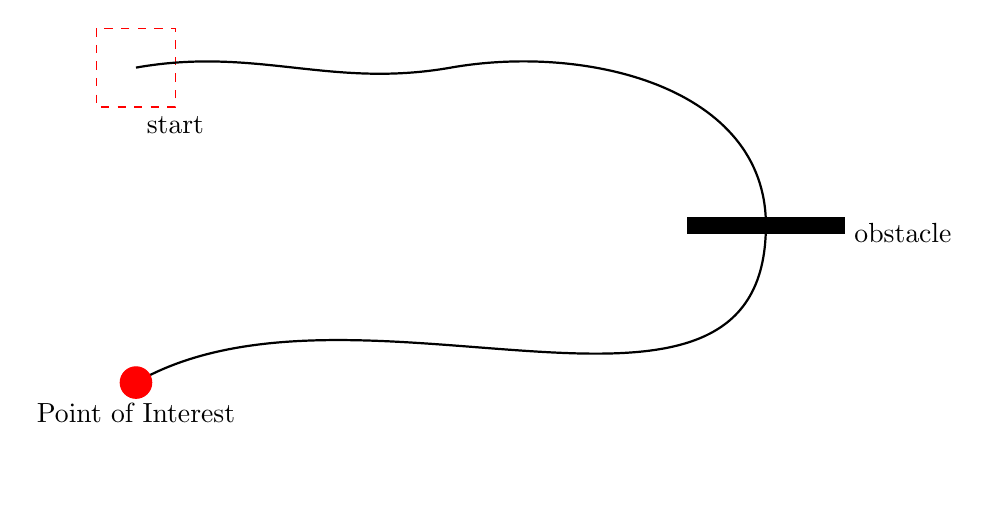
\begin{tikzpicture}
            % draw a red rectangle
            \draw [red, dashed] (-2.5, 2.5) rectangle (-1.5, 1.5) node [black, below] {start};
            \draw [thick] (-2, 2) % draw a line
            to [out=10, in=190] (2, 2)
            to [out=10, in=90] (6, 0)
            to [out=-90, in=30] (-2, -2);
            \draw [fill] (5, 0.1) rectangle (7, -0.1) node [black, right] {obstacle};
            \draw [red, fill] (-2, -2) circle [radius=0.2] node [black, below=4] {Point of Interest};
        \end{tikzpicture}
        \caption{Example graphic made with tikz}
        \label{fig:graphc1}
    \end{center}
\end{figure}


\subsection{HyperLink}
This is google link: \href{www.google.com}{Google} \\
Embed a bare URL \url{www.google.com}

\subsection{List}
Will introduce the unordered list first
\begin{itemize}
    \item[--] this is unordered list % from bullet to dash
    \item environment \textbf{itemize}
    \item[$\ast$] asterisk
\end{itemize}
Ordered list is in \textbf{enumerate}
\begin{enumerate}
    \item B
    \item A
    \item C
\end{enumerate}
Following is nested list
\begin{enumerate}
	\item One
    \begin{enumerate}
    	\item Two
        \item Three
        \item Four
    \end{enumerate}
    \item Five
    \item Six
\end{enumerate}

\newpage
\bibliography{reference}
\bibliographystyle{ieeetr}

%% example for footnote citation
%\newpage
%\printbibliography

\end{document}